\documentclass[AMA,STIX1COL]{WileyNJD-v2}

\articletype{Research Article}

\received{26 April 2016}
\revised{6 June 2016}
\accepted{6 June 2016}

%\raggedbottom

%\usepackage{booktabs}

\let\procedure\relax
\let\endprocedure\relax

%\usepackage[ruled]{algorithm2e} % For algorithms
\usepackage[noline, noend, nofillcomment]{algorithm2e}
%\usepackage[noline, noend, nofillcomment, linesnumbered]{algorithm2e}
%    \setlength{\algomargin}{0em}
    \SetArgSty{textnormal}
%    \SetNoFillComment
%    \newcommand{\Xcmfont}[1]{\texttt{\footnotesize{#1}}}\SetCommentSty{Xcmfont}
\renewcommand{\algorithmcfname}{ALGORITHM}
%\SetAlFnt{\small}
%\SetAlCapFnt{\small}
%\SetAlCapNameFnt{\small}
%\SetAlCapHSkip{0pt}
\IncMargin{-\parindent}

\usepackage[utf8]{inputenc}
\usepackage{amsmath,amssymb,amsfonts}
\usepackage{accents}
\usepackage{mathtools}
\usepackage{graphicx}
\usepackage{enumitem}
\usepackage[justification=centering]{caption}
\usepackage{url}

\newcommand{\Xl}{\langle}
\newcommand{\Xr}{\rangle}
\newcommand{\Xm}{\langle\!\rangle}
\newcommand{\Xset}{\!\leftarrow\!}
\newcommand{\Xund}{\rule{.4em}{.4pt}}
\newcommand{\Xlb}{[\![}
\newcommand{\Xrb}{]\!]}
\newcommand{\Xmap}{\!\mapsto\!}
\newcommand{\XB}{\mathcal{B}}
\newcommand{\XD}{\mathcal{D}}
\newcommand{\XE}{\mathcal{E}}
\newcommand{\XF}{\mathcal{F}}
\newcommand{\XI}{\mathcal{I}}
\newcommand{\XL}{\mathcal{L}}
\newcommand{\XN}{\mathcal{N}}
\newcommand{\XM}{\mathcal{M}}
\newcommand{\XO}{\mathcal{O}}
\newcommand{\XP}{\mathcal{P}}
\newcommand{\XR}{\mathcal{R}}
\newcommand{\XS}{\mathcal{S}}
\newcommand{\XT}{\mathcal{T}}
\newcommand{\XX}{\mathcal{X}}
\newcommand{\YB}{\mathbb{B}}
\newcommand{\YF}{\mathbb{F}}
\newcommand{\YN}{\mathbb{N}}
\newcommand{\YT}{\mathbb{T}}
\newcommand{\YQ}{\mathbb{Q}}
\newcommand{\YZ}{\mathbb{Z}}

\newcommand{\Xstirling}[2]{\genfrac{\{}{\}}{0pt}{}{#1}{#2}}
\newcommand*{\Xbar}[1]{\overline{#1\vphantom{\bar{#1}}}}

\setlist{nosep}
%\setlength{\parskip}{0.5em}

\newenvironment{Xfig}
    {\par\medskip\noindent\minipage{\linewidth}\begin{center}}
    {\end{center}\endminipage\par\medskip}
\newenvironment{Xtab}
    {\par\medskip\noindent\minipage{\linewidth}\begin{center}}
    {\end{center}\endminipage\par\medskip}

%\setlength{\parindent}{0pt}

%\theoremstyle{definition}
\newtheorem{Xdef}{Definition}
\newtheorem{XThe}{Theorem}
\newtheorem{XLem}{Lemma}
\newtheorem{Xobs}{Observation}


\begin{document}

\title{POSIX Disambiguation on Tagged NFA}

\author[1]{Angelo Borsotti}
\author[2]{Ulya Trofimovich}

\address[1]{\email{angelo.borsotti@mail.polimi.it}}
\address[2]{\email{skvadrik@gmail.com}}

\abstract[Summary]{
We give an algorithm for POSIX submatch extraction in regular expressions.
Our work is based on the prior work of Okui and Suzuki, with a number of improvements.
First, the new algorithm can handle bounded repetition.
Second, it explores only a part of the regular expression structure
necessary to disambiguate submatch extraction,
which reduces the overhead for expressions with few submatch groups.
Third, we use Thompson automaton instead of position automaton
and give an efficient algorithm for $\epsilon$-closure construction,
which allows us to skip the pre-processing step of Okui-Suzuki algorithm.
%based on the Goldberg-Radzik shortest path finding algorithm.
The complexity of our algorithm is $O(nv^2e)$ in general and $O(nve)$ for regular expression without $\epsilon$-loops,
where $n$ is the input length, $v$ is the number of states and $e$ is the number of transitions in the automaton.
}

\keywords{Lexical Analysis, Regular Expressions, Submatch Extraction, POSIX}

%\jnlcitation{\cname{
%\author{U. Trofimovich},
%(\cyear{2017}),
%\ctitle{Fast Submatch Extraction in Lexer Generators},
%\cjournal{Q.J.R. Meteorol. Soc.},
%\cvol{2017;00:1--6}.}

\maketitle

\section*{Introduction}

\iffalse

     Yes, I know --- you've always been after building full parse trees,


This is true, but the issue here is different. It is a matter of RE syntax and its interpretation.
As you know, there are two views of REs: the one of Kleene (the theoretical computer science one), and the
one of RE libraries. The first  (see Kleene, Stephen C. (1951). Shannon, Claude E.; McCarthy, John, eds.
Representation of Events in Nerve Nets and Finite Automata (PDF). Automata Studies. Princeton University
Press. pp. 3–42) has no notion of submatches and capturing parentheses. Indeed, parentheses in it
are seen as in math, i.e. having no other significance than a means of changing the precedence of
operators. In it then, r* and (r)* are the same.
In the RE libraries view, this could be different. E.g. in the POSIX standard (the first, Chapter 9) the definition
of "matching" (9.4.6) refers always to "ERE matching a single character or an ERE enclosed in parentheses"
making thus no distiction between r* and (r)*. What makes the distinction is the POSIX standard for regex().
Actually, tagged automata depart from regex() since they allow to get the match of any part of a string be it
derived from a capturing group or not.
I think that we can do what we want since we are not presenting a paper that describes an implementation of
regex(). I have no problems in making the distinction; it is a valid choice much the same as the other one.
After all, since we are not describing an implementation of regex(), this distinction does not make much
a difference (apart perhaps a level in the pictures of trees, and some tweaks in the proofs).

\fi

Description of Okui algorithm.
\\ \\
Contributions.
%\begin{itemize}
%    \item
%    \item
%\end{itemize}
\\ \\
The rest of this paper is arranged as follows.

\section{Regular Expressions as Parse Trees}

We define regular expressions as follows\footnote{
Regular expressions originate in the work of Kleene\cite{Kle51}.
A rigorous definition of regular expressions is given in terms of Kleene algebra\cite{Koz94}.}:

    \begin{Xdef}
    \emph{Regular expressions (RE)} over finite alphabet $\Sigma$, denoted $\XE_\Sigma$, are:
    \begin{enumerate}
        \item Atomic RE:
%          \emph{empty set} $\emptyset \in \XE_\Sigma$,
          \emph{empty word} $\epsilon \in \XE_\Sigma$ and
          \emph{unit word} $\alpha \in \XE_\Sigma$, where $\alpha \in \Sigma$.
        \item Compound RE: if $e_1, e_2 \in \XE_\Sigma$, then
          \emph{union} $e_1 | e_2 \in \XE_\Sigma$,
          \emph{product} $e_1 e_2 \in \XE_\Sigma$,
          \emph{repetition} $e_1^{n, m} \in \XE_\Sigma$ (where $0 \leq n \leq m \leq \infty$), and
          \emph{submatch group} $(e_1) \in \XE_\Sigma$.
    \end{enumerate}
    \end{Xdef}

This definition is somewhat different from the usual definition\cite{HU90}\cite{SS88};
it is adapted to the POSIX standard.
First, we consider parentheses as a distinct construct: in POSIX $(e)$ is semantically different from $e$.
Second, we use generalized repetition $e^{n, m}$ instead of iteration $e^*$:
expressing repetition in terms of iteration and product requires duplication of the subexpression,
which may change semantics: e.g. in POSIX $(e)(e)$ is not the same as $(e)^{2,2}$.
As usual, we assume that repetition has precedence over product and product over union,
and parentheses may be used to override it (all parentheses are capturing).
%Additionally, we use the following shortcut notation:
%$e^*$ for $e^{0,\infty}$,
%$e^+$ for $e^{1,\infty}$,
%$e^?$ for $e^{0,1}$,
%and $e^n$ for $e^{n,n}$.
% %\\
% %
% %One possible interpretation of RE is the \emph{tree} interpretation,
% %in which every RE denotes a set of \emph{parse trees}.
\\

First of all, we rewrite RE in a form where, instead of submatch groups,
every subexpression has a pair of integer indices indicating its significance for submatch extraction.
Second index indicates \emph{explicit} submatch groups:
its value is equal to the number of submatch group, otherwize zero.
First index is like the second one, but it also accounts for \emph{implicit} submatch groups:
subexpressions that are not themselves parenthesized, but have nested or sibling parenthesized subexpressions.
If both indices are zero, it means that the subexpression is ignored from submatch extraction perspective.
If only the second index is zero, it means that the subexpression itself is not interesting,
but some other submatch groups depend on it.
Explicit indices are convenient because they allow us to consider individual subexpressions
without loosing submatch context of the whole RE.
We call this representation \emph{regular expression trees}.
An example of RT can be seen on figure \ref{fig_parse_trees}.

    \begin{Xdef}
    \emph{Regular expression trees (RT)} over finite alphabet $\Sigma$, denoted $\XR_\Sigma$, are:
    \begin{enumerate}
        \item Atomic RT:
          \emph{empty tree} $(i, j, \epsilon) \in \XR_\Sigma$ and
          \emph{unit tree} $(i, j, \alpha) \in \XR_\Sigma$, where $\alpha \in \Sigma$ and $i, j \in \YZ$.

        \item Compound RT: if $r_1, r_2 \in \XR_\Sigma$ and $i, j \in \YZ$, then
          \emph{union} $(i, j, r_1 \mid r_2) \in \XR_\Sigma$,
          \emph{product} $(i, j, r_1 \cdot r_2) \in \XR_\Sigma$ and
          \emph{repetition} $(i, j, r_1^{n, m}) \in \XR_\Sigma$ (where $0 \leq n \leq m \leq \infty$).
    \end{enumerate}
    \end{Xdef}

Function $RT : \XE_\Sigma \rightarrow \XR_\Sigma$ transforms RE into RT.
It is defined via a composition of two functions,
$mark$ that transforms RE into RT with submatch indices in the boolean range $\{0, 1\}$
(indicating if the given subexpression is an implicit/explicit submatch group),
and $enum$ that substitutes boolean indices with the actual numbers:
$RT(e) = r$ where $(\Xund, \Xund, r) = enum(1, 1, mark(e))$.
%
    \begin{align*}
    &\begin{aligned}
        mark &: \XE_\Sigma \longrightarrow \XR_\Sigma \\
        mark &(x) = (0, 0, x) \\
            &\text{where } x \in \{\epsilon, \alpha\}
        \\
        %
        mark &(e_1 \circ e_2) = (i, 0,
            (i, j_1, r_1) \circ
            (i, j_2, r_2)
            ) \\
            &\text{where } \circ \in \{|,\cdot\} \\
            &\space{\hphantom{where }}(i_1, j_1, r_1) = mark(e_1) \\
            &\space{\hphantom{where }}(i_2, j_2, r_1) = mark(e_2) \\
            &\space{\hphantom{where }}i = i_1 \vee i_2 \\
        %
        mark &(e^{n, m}) = (i, 0, (i, j, r)^{n, m}) \\
            &\text{where } (i, j, r) = mark(e) \\
        %
        mark &((e)) = (1, 1, r) \\
            &\text{where } (\Xund, \Xund, r) = mark(e)
    \end{aligned}
    %
    &&\begin{aligned}
        enum &: \YZ \times \YZ \times \XR_\Sigma \longrightarrow \YZ \times \YZ \times \XR_\Sigma \\
        enum &(\bar{i}, \bar{j}, (i, j, x)) = (\bar{i} + i, \bar{j} + j, (\bar{i} \times i, \bar{j} \times j, x)) \\
            &\text{where } x \in \{\epsilon, \alpha\}
        \\
        enum &(\bar{i}, \bar{j}, (i, j, r_1 \circ r_2)) = (i_2, j_2, (\bar{i} \times i, \bar{j} \times j, \bar{r}_1 \circ \bar{r}_2)) \\
            &\text{where } \circ \in \{|,\cdot\} \\
            &\space{\hphantom{where }}(i_1, j_1, \bar{r}_1) = enum(\bar{i} + i, \bar{j} + j, r_1) \\
            &\space{\hphantom{where }}(i_2, j_2, \bar{r}_2) = enum(i_1, j_1, r_2)
        \\
        enum &(\bar{i}, \bar{j}, (i, j, r^{n,m})) = (i_1, j_1, (\bar{i} \times i, \bar{j} \times j, \bar{r}^{n,m})) \\
            &\text{where }
                (i_1, j_1, \bar{r}) = enum(\bar{i} + i, \bar{j} + j, r)
    \end{aligned}
    \end{align*}

RE and RT are equivalent representations
(we can transform RT back to RE
by erasing all submatch indices
and adding parentheses around subexpressions with nonzero explicit submatch index).
Each RT (and the corresponding RE) denotes a set of \emph{parse trees}.
Tree nodes inherit implicit submatch index from RT nodes
(we mark it with superscript).
Explicit submatch index is dropped, as there is no use for it in the context of parse trees (in the current paper).

    \begin{Xdef}
    \emph{Parse trees (PT)} over finite alphabet $\Sigma$, denoted $\XT_\Sigma$, are:
    \begin{enumerate}
        \item Atomic PT:
          \emph{nil tree} ${\varnothing}^i \in \XT_\Sigma$,
          \emph{empty tree} ${\epsilon}^i \in \XT_\Sigma$ and
          \emph{unit tree} ${\alpha}^i \in \XT_\Sigma$, where $\alpha \in \Sigma$ and $i \in \YZ$.
        \item Compound PT: if $t_1, \dots, t_n \in \XT_\Sigma$, where $n \geq 1$, and $i \in \YZ$, then
          ${T}^i(t_1, \dots, t_n) \in \XT_\Sigma$.
    \end{enumerate}
    \end{Xdef}

Note that our parse trees are different from \ref{OS13}:
we have a \emph{nil} tree (a placeholder for absent alternative and zero repetitions)
and do not differentiate between various kinds of compound trees.
Tree interpretation of RT is given by operator $PT: \XR_\Sigma \rightarrow 2^{\XT_\Sigma}$:
    \begin{align*}
        PT\big((i, \Xund, \epsilon)\big) &= \{ {\epsilon}^{i} \}
        \\
        PT\big((i, \Xund, \alpha)\big) &= \{ {\alpha}^{i} \}
        \\
        PT\big((i, \Xund, (i_1, j_1, r_1) \mid (i_2, j_2, r_2))\big) &=
            \big\{ {T}^{i}(t, \varnothing^{i_2}) \mid t \in PT\big((i_1, j_1, r_1)\big) \big\} \cup
            \big\{ {T}^{i}(\varnothing^{i_1}, t) \mid t \in PT\big((i_2, j_2, r_2)\big) \big\}
        \\
        PT\big((i, \Xund, (i_1, j_1, r_1) \cdot (i_2, j_2, r_2))\big) &=
            \big\{ {T}^{i}(t_1, t_2) \mid
                t_1 \in PT\big((i_1, j_1, r_1)\big),
                t_2 \in PT\big((i_2, j_2, r_2)\big)
            \big\} \\
        PT\big((i, \Xund, (i_1, j_1, r_1)^{n, m})\big) &=
            \begin{cases}
                \big\{ {T}^{i}(t_1, \dots, t_m) \mid t_i \in PT\big((i_1, j_1, r_1)\big) \;
                    \forall i = \overline{1, m} \big\} \cup \{ {T}^{i}(\varnothing^{i_1}) \} &\text{if } n = 0 \\
                \big\{ {T}^{i}(t_n, \dots, t_m) \mid t_i \in PT\big((i_1, j_1, r_1)\big) \;
                    \forall i = \overline{n, m} \big\} &\text{if } n > 0
            \end{cases}
    \end{align*}

The \emph{string} induced by a tree $t$, denoted $str(t)$, is the concatenation of all alphabet symbols in the left-to-right traversal of $t$.
For an RT $r$ and a string $w$, we write $PT(r, w)$ to denote the set $\{ t \in PT(r) \mid str(t) = w \}$
(note that this set is potentially infinite).
\\

Following \cite{OS13}, we assign \emph{positions} to the nodes of RT and PT.
The root position is $\Lambda$, and position of the $i$-th subtree of a tree with position $p$ is $p.i$.
The \emph{length} of position $p$, denoted $|p|$, is defined as $0$ for $\Lambda$ and $|p| + i$ for $p.i$.
%The set of all positions is denoted $\XP$.
The subtree of a tree $t$ at position $p$ is denoted $t|_p$.
Position $p$ is a \emph{prefix} of position $q$ iff $q = p.p'$ for some $p'$,
and a \emph{proper prefix} if additionaly $p \neq q$.
Position $p$ is a \emph{sibling} of position $q$ iff $q = q'.i, p = q'.j$ for some $q'$ and $i,j \in \YN$.
Positions are ordered lexicographically, as in \ref{OS13}.
The set of all positions of a tree $t$ is denoted $Pos(t)$.
The set of \emph{submatch positions} of a tree $t$
is the subset of $Pos(t)$ containing positions of subtrees with nonzero submatch index:
$Sub(t) = \{ p \mid \exists i \neq 0, s: t|_p = s^i \}$.
Examples of parse trees can be seen on figure \ref{fig_parse_trees}.

\begin{figure}\label{fig_parse_trees}
\includegraphics[width=\linewidth]{img/trees.pdf}
\caption{
RT and examples of PT for RE $(\epsilon|a^{0,\infty})(a|\epsilon)^{0,\infty}$ and string $a$.\\
Order:
$s <_1 t$,
$s <_1 u$,
$u <_{2.2} t$.
Okui-Suzuki order:
$s <^{os}_1 t$,
$s <^{os}_1 u$,
$t <^{os}_{1.1} u$.
}
\end{figure}

%    \begin{Xdef}
%    \emph{Lexicographic order on positions.}
%    Given positions $p = p_1. \dots .p_n$ and $q = q_1. \dots q_m$, we say that $p < q$ iff either
%    $\exists k < min(n,m) : p_k < q_k$,
%    or $n < m \wedge p_i = q_i \; \forall i = \overline{1, n}$.
%    \end{Xdef}

    \begin{Xdef}\label{norm_of_parse_tree}
    The \emph{norm} of PT $t$ at position $p$ is:
    $$
    \|t\|_p =
        \begin{cases}
            -1          &\text{if } \exists i \neq 0, s = \varnothing: t|_p = s^i \\
            |str(t|_p)| &\text{if } \exists i \neq 0, s \neq \varnothing: t|_p = s^i \\
            \infty      &\text{otherwise}
        \end{cases}
    $$
    \end{Xdef}

In other words, the norm is infinite for all positions not in $Sub(t)$,
and for positions in $Sub(t)$ it depends on the form of subtree:
for nil subtrees it equals $-1$,
and for other subtrees it equals the number of symbols.
We shorten $\|t\|_\Lambda$ as $\|t\|$.

    \begin{Xdef}\label{order_on_parse_trees}
    \emph{Order on parse trees.}
    Given parse trees $t, s \in PT(e, w)$, we say that $t <_p s$ w.r.t. \emph{desision position} $p$ % $p \in Sub(t) \cup Sub(s)$
    iff $\|t\|_p > \|s\|_p$ and $\|t\|_q = \|s\|_q \; \forall q < p$.
    (Note that we do not explicitly demand that $p, q \in Sub(t) \cup Sub(s)$:
    if this is not the case, the norms of both subtrees are $\infty$ and thus equal.)
    We say that $t < s$ iff $t <_p s$ for some $p$.
    If neither $t < s$, nor $s < t$, we say that $t$ and $s$ are \emph{incomparable}: $t \sim s$.
    \end{Xdef}

    \begin{XLem}\label{lemma_ptorder_antisymmetry}
    Order on parse trees is antisymmetric: if $t < s$, then $s \not< t$.
    \\
    Proof.
    Suppose, on the contrary, that $t <_p s$ and $s <_q t$ for some $p$, $q$.
    Without loss of generality let $p \leq q$.
    On one hand $t <_p s$ implies $\|t\|_p > \|s\|_p$.
    On the other hand $s <_q t$ implies $\|t\|_p \leq \|s\|_p$.
    Contradiction.
    $\square$
    \end{XLem}

    \begin{XLem}\label{lemma_ptorder_transitivity}
    Order on parse trees is transitive: if $t < s$ and $s < u$, then $t < u$.
    \\
    Proof.
    Let $t <_p s$ and $s <_q u$ for some positions $p$, $q$, and let $r = min (p, q)$.

    \medskip

    First, we show that $\|t\|_r > \|u\|_r$.
    If $p \leq q$, we have $\|t\|_p > \|s\|_p$ (implied by $t <_p s$)
    and $\|s\|_p \geq \|u\|_p$ (implied by conjunction $s <_q u \wedge p \leq q$),
    therefore $\|t\|_p > \|u\|_p$.
    Otherwise $p > q$, we have $\|s\|_q > \|u\|_q$ (implied by $s <_q u$)
    and $\|t\|_q = \|s\|_q$ (implied by conjunction $t <_p s \wedge q < p$),
    therefore $\|t\|_q > \|u\|_q$.

    \medskip

    Second, we show that $\forall r' < r$ it holds that $\|t\|_{r'} = \|u\|_{r'}$.
    We have $\|t\|_{r'} = \|s\|_{r'}$ (implied by conjunction $t <_p s \wedge r' < p$)
    and $\|s\|_{r'} = \|u\|_{r'}$ (implied by conjunction $s <_q u \wedge r' < q$),
    therefore $\|t\|_{r'} = \|u\|_{r'}$.
    $\square$
    \end{XLem}

    \begin{XLem}\label{incomparability_equivdef}
    $t \sim s \Leftrightarrow \; \forall p : \|t\|_p = \|s\|_p$.
    \\
    Proof.

    $\Rightarrow$. %First, we show $t \sim s \Rightarrow \forall p : \|t\|_p = \|s\|_p$.
    Suppose, on the contrary, that $\exists p = min \{ q \mid \|t\|_q \neq \|s\|_q \}$,
    then either $t <_p s$ (if $\|t\|_p > \|s\|_p$), or $s <_p t$ (if $\|t\|_p < \|s\|_p$).
    Both cases contradict $t \sim s$.

    \medskip

    $\Leftarrow$.
    $\forall p : \|t\|_p = \|s\|_p$ implies
    $\nexists p : t <_p s$ and $\nexists q : s <_q t$,
    which implies $t \sim s$.
    $\square$
    \end{XLem}

    \begin{XLem}\label{lemma_ptorder_transitivity_of_incomparability}
    Incomparability relation on parse trees is transitive: if $t \sim s$ and $s \sim u$, then $t \sim u$.
    \\
    Proof.
    By lemma \ref{incomparability_equivdef} we have
    $t \sim s \Rightarrow \forall p : \|t\|_p = \|s\|_p$ and
    $s \sim u \Rightarrow \forall p : \|s\|_p = \|u\|_p$,
    therefore by lemma \ref{incomparability_equivdef} $\forall p : \|t\|_p = \|u\|_p \Rightarrow t \sim u$.
    $\square$
    \end{XLem}

    \begin{XThe}
    Relation $<$ is strict weak order on parse trees.
    \\
    \medskip
    Proof.
    Follows from
    lemma \ref{lemma_ptorder_antisymmetry},
    lemma \ref{lemma_ptorder_transitivity} and
    lemma \ref{lemma_ptorder_transitivity_of_incomparability}.
    $\square$
    \end{XThe}

If in Definition \ref{norm_of_parse_tree} and Definition \ref{order_on_parse_trees}
we use $Pos(t)$ instead of $Sub(t)$, then our strict weak order $<$
coincides with Okui-Suzuki strict total order on parse trees \cite{OS13} (we denote the latter with $<^{os}$).
%TODO: the existense of minimal element remains to be shown, as we don't have CPT.
While it is not true in general that $<^{os}$ is an extension of $<$
(see the counterexample on figure \ref{fig_parse_trees}),
the two orders are compatible in the sense that the $<^{os}$-minimal tree
is included in the class of $<$-minimal trees.
Intuitively, this means that if we keep ``refining'' submatch detalization
by adding parentheses in subexpressions,
we will gradually narrow down the class of $<$-minimal trees,
until we are left with a single $<^{os}$-minimal tree.
Theorem \ref{lemma_order_compat} shows this,
and lemma \ref{lemma_subtrees} shows that comparison of subtrees is justified
if the norms of all preceding submatch positions are equal.

    \begin{XLem}\label{lemma_subtrees}
    If $t, s \in PT(r, w)$ and $\exists p \in Sub(t) \cup Sub(s)$ such that $\|t\|_q = \|s\|_q \; \forall q \leq p$,
    then $\exists \widetilde{r}, \widetilde{w} : t|_p, s|_p \in PT(\widetilde{r}, \widetilde{w})$.
    \\
    Proof.
    By induction on position $p$.

    \medskip

    Induction basis: the case of $p = \Lambda$ is trivial: let $\widetilde{r} = r$, $\widetilde{w} = w$.

    \medskip

    Induction step: we have $|p| > 0$, let $p = p'.i$, where $i \in \YN$.
    Let $t' = t|_{p'} = P(t_1, \dots, t_n)$,
        $s' = s|_{p'} = P(s_1, \dots, s_m)$.
    By induction hypothesis $\exists r', w' : t', s' \in PT(r', w')$,
    where $w' = str(t_1) \dots str(t_n) = str(s_1) \dots str(s_m)$.

    \medskip

    Next, we show that $str(t_i) = str(s_i)$.
    It must be that $i \in Sub(s') \cap Sub(t')$,
    otherwise only one of $\|t'\|_i$, $\|s'\|_i$ is $\infty$,
    which contradicts lemma condiiton $\|t\|_p = \|s\|_p$.
    Consider position $j \leq i$.
    Because the set of submatch positions contains siblings, we have $j \in Sub(s') \cap Sub(t')$.
    Consequently, $\|t'\|_j = |str(t_j)|$ and $\|s\|_j = |str(s_j)|$.
    By lemma condition we have $\|t\|_{p'.j} = \|s\|_{p'.j}$,
    therefore $\|t'\|_j = \|s'\|_j$,
    therefore $|str(t_j)| = |str(s_j)|$.
    Because $str(t_1) \dots str(t_n) = str(s_1) \dots str(s_m)$,
    we have $str(t_i) = str(s_i)$.

    \medskip

    Now, let $\widetilde{w} = str(t_i)$.
    If $r' = r_1|r_2$ or $r' = r_1 r_2$, let $\widetilde{r} = r_i$.
    Otherwise, $r' = r_1^{k,l}$, let $\widetilde{r} = r_1$.
    $\square$
    \end{XLem}

    \begin{XThe}\label{lemma_order_compat}
    For a set of parse trees $P = PT(r, w)$,
    let $s$ be the $<^{os}$-minimal tree,
    and $P_{min} = \{ t \in P \mid \forall u \in P : t = u \vee t < u \}$ the class of $<$-minimal trees.
    Then $s \in P_{min}$.
%    let $s$ be the $\prec$-minimal tree: $s = min_{<^{os}} P$,
%    and $t$ one of the $<$-minimal trees: $t \in \{ u \in P \mid \forall u' \in P : u = u' \vee u < u' \}$.
%    Then $s \sim t$.
    \\
    Proof.

    Consider any $t \in P_{min}$.
    For each position $p \in Sub(t)$ which is not itself a prefix of another position in $Sub(t)$,
    consider subtree $t' = t|_p$.
    It is a parse tree for some subexpression $r'$ and substring $w'$: $t' \in PT(r', w')$.
    Let $t''$ be the $<^{os}$-minimal tree in $PT(r', w')$ and substitute $t'$ with $t''$ in $t$.
    (Note that substitutions are independent and can be performed in any order.)
    Let $u$ be the tree resulting from all such substitutions.
    By lemma \ref{incomparability_equivdef} we have $u \sim t$
    (substitutions preserve the norm of subtrees at positions in $Sub(t)$),
    and so $u \in P_{min}$.

    \medskip

    Next, we show that $u = s$.
    Suppose, on the contrary, that $u \neq s$.
    Then, on one hand, $u <_q s$ for some $q \in Sub(s) \cup Sub(u)$ (because $u \in P_{min}$).
    On the other hand, $s <^{os}_p u$ for some $p \in Pos(s) \cup Pos(u)$, such that $p < q$ (because $s$ is $<^{os}$-minimal).
    Let $p = p'.p''$, where $p'$ is the longest prefix of $p$ in $Sub(s) \cup Sub(u)$.
    It must be $\|u\|_{q'} = \|s\|_{q'} \forall q' \leq p'$ (because $p' < q$ and $u <_q s$),
    and $p' \in Sub(u)$ (otherwise $\|u\|_{p'} = \infty \neq \|s\|_{p'}$).
    Now, by lemma \ref{lemma_subtrees} we have $\exists r', w' : u|_{p'}, s|_{p'} \in PT(r', w')$,
    therefore $s <^{os}_{p'.p''} u$ implies $s|_{p'} <^{os}_{p''} u|_{p'}$.
    But $p' \in Sub(u)$ and $p'$ is not itself a prefix of another position in $Sub(u)$,
    therefore $u|_{p'}$ is $<^{os}$-minimal by construction of $u$.
    Contradiction.
    $\square$
    \end{XThe}

\section{Parenthezised expressions}

In this section we introduce linearised representation of parse trees: \emph{parenthesized expressions}.
%The structure of the section follows \cite{OS13},
%however there are subtle, but important differences in some of the definitions and proofs.

    \begin{Xdef}
    \emph{Parenthesized expressions (PE)} over finite alphabet $\Sigma$, denoted $\XP_\Sigma$, are:
    \begin{enumerate}
        \item Atomic PE:
          \emph{nil expression} $\Xm \in \XP_\Sigma$,
          \emph{empty expression} $\epsilon \in \XP_\Sigma$ and
          \emph{unit expression} $a \in \XP_\Sigma$, where $\alpha \in \Sigma$.
        \item Compound PE: if $e_1, e_2 \in \XP_\Sigma$, then
            $e_1 e_2 \in \XP_\Sigma$ and
            $\Xl e_1 \Xr \in \XP_\Sigma$.
    \end{enumerate}
    \end{Xdef}

Parenthesis $\Xl$ is called \emph{opening} and
parenthesis $\Xr$ is called \emph{closing};
the \emph{nil}-parenthesis $\Xm$ is both opening and closing.
The \emph{height} of parenthesis in a PE is the number of preceding opening parentheses (including this one)
minus the number of preceding closing parentheses (including this one).
For convenience we sometimes explicitly denote height with subscript:
this allows us to consider (not necessarily correctly nested) fragments of the given PE in isolation,
without losing the context of the whole PE.
However, height is not a part of parenthesis itself
and is not taken into account when comparing the elements of PE.
Function $\Phi : \YZ \times \XT_\Sigma \rightarrow \XP_\Sigma$ transforms PT into PE:
    $$
    \Phi_{h}(t^{i}) = \begin{cases}
        str(t^{i})                                            &\text{if } i = 0 \\
        \Xm_h                                                 &\text{if } i \neq 0 \wedge t = \varnothing \\
        \Xl_{h+1} \Xr_h                                       &\text{if } i \neq 0 \wedge t = \epsilon \\
        \Xl_{h+1} a \Xr_h                                     &\text{if } i \neq 0 \wedge t = a \in \Sigma \\
        \Xl_{h+1} \Phi_{h+1}(t_1) \dots \Phi_{h+1}(t_n) \Xr_h &\text{if } i \neq 0 \wedge t = T(t_1, \dots, t_n)
    \end{cases}
    $$

For a given RT $r$ and string $w$, the set $\big\{ \Phi_{0}(t) \mid t \in PT(r, w) \big\}$ is denoted $PE(r, w)$.
If $\alpha, \beta \in PE(r, w)$ for some $r$ and $w$, we say that $\alpha$ and $\beta$ are \emph{comparable}.
%
For PE $\alpha$, $\beta$,
$\alpha \sqcap \beta$ denotes the longest common prefix of $\alpha$ and $\beta$,
$\alpha \backslash \beta$ denotes the suffix of $\alpha$ after removing $\alpha \sqcap \beta$,
$lastht(\alpha)$ denotes the height of the last parenthesis in $\alpha$ or $\infty$ if $\alpha$ is empty or begins with a letter,
$minht(\alpha)$ denotes the minimal height of parenthesis in $\alpha$ or $\infty$ if $\alpha$ is empty or begins with a letter,
$first(\alpha)$ denotes the first parenthesis in $\alpha$ or $\bot$ if $\alpha$ is empty or begins with a letter.
Each PE $\alpha$ can be represented as $\alpha_0 a_1 \alpha_1 \dots a_n \alpha_n$,
where $\alpha_i$ is the $i$-th \emph{frame} --- the possibly empty sequence of parentheses between
subsequent alphabet symbols $a_i$ and $a_{i+1}$ or the beginning or end of $\alpha$.
Note that comparable PE have the same number of frames.
For distinct comparable PE $\alpha$, $\beta$
the index of the first distinct pair of frames is called \emph{fork}.

    \begin{Xdef}
    Let $\alpha$, $\beta$ be distinct comparable PE, such that
    $\alpha = \alpha_0 a_1 \alpha_1 \dots a_n \alpha_n$,
    $\beta = \beta_0 a_1 \beta_1 \dots a_n \beta_n$ and $k$ is the fork.
    We define $trace (\alpha, \beta)$ as the sequence $(\rho_0, \dots, \rho_n)$, where:
    $$
    \rho_i = \begin{cases}
        -1 &\text{if } i < k \\
        min (lastht (\alpha_i \sqcap \beta_i), minht(\alpha_i \backslash \beta_i)) &\text{if } i = k \\
        min (\rho_{i-1}, minht(\alpha_i)) &\text{if } i > k
    \end{cases}
    $$
    We write $traces(\alpha, \beta)$ to denote $\big( trace (\alpha, \beta), trace (\beta, \alpha) \big)$.
    $\square$
    \end{Xdef}

    \begin{Xdef}\label{prec1}
    Let $\alpha$, $\beta$ be comparable PE and
    $traces(\alpha, \beta) = \big( (\rho_0, \dots, \rho_n), (\rho'_0, \dots, \rho'_n) \big)$.
    The \emph{longest-precedence} relation $\sqsubset$ is defined as
    $\alpha \sqsubset \beta \Leftrightarrow \exists i \leq n:
        \big( \rho_i > \rho'_i \big) \wedge
        \big( \rho_j = \rho'_j \; \forall j > i \big)$.
%    $$
%        \alpha \sqsubset \beta \quad \Leftrightarrow \quad \exists i \leq n:
%        \prescript{}{\wedge}{\left[
%            \begin{aligned}
%                &\rho_i > \rho'_i \\
%                &\forall j > i: \rho_j = \rho'_j
%            \end{aligned}
%        \right.}
%    $$
    If neither $\alpha \sqsubset \beta$, nor $\beta \sqsubset \alpha$,
    then $\alpha$, $\beta$ are \emph{longest-equivalent}: $\alpha \sim \beta$
    (note that in this case $\rho_i > \rho'_i \; \forall i = \overline {1, n}$).
    \end{Xdef}

    \begin{Xdef}\label{prec2}
    Let $\alpha$, $\beta$ be comparable PE, and let
    $x = first (\alpha \backslash \beta)$,
    $y = first (\beta \backslash \alpha)$.
    The \emph{leftmost-precedence} relation $\subset$ is defined as
    $\alpha \subset \beta \Leftrightarrow x < y$, where
    the set of possible values of $x$ and $y$ is ordered as follows:
    $\bot < \Xr < \Xl < \Xm$.
%    Let $\alpha$, $\beta$ be comparable PE, and let
%    $x = first (\alpha \backslash \beta)$,
%    $y = first (\beta \backslash \alpha)$.
%    The \emph{leftmost-precedence} relation $\subset$ is defined as follows:
%    $\alpha \subset \beta \Leftrightarrow
%    \big(x = \bot \wedge y \not= \bot \big) \vee
%    \big(x = \Xr \wedge y \not= \bot \big) \vee
%    \big(x = \Xl \wedge y = \bar{\Xl} \big)$.
%
%    $$
%        \alpha \subset \beta \quad \Leftrightarrow \quad
%        \prescript{}{\vee \;}{\left[
%            \begin{aligned}
%                &x = \bot   &&\wedge && y \not= \bot \\
%                &x = \Xr    &&\wedge && y \not= \bot \\
%                &x = \Xl    &&\wedge && y = \bar{\Xl}
%            \end{aligned}
%        \right.}
%    $$
    \end{Xdef}

    \begin{Xdef}\label{pe_order}
    The \emph{longest-leftmost-precedence} relation $<$ on comparable PE is defined as
    $\alpha < \beta \Leftrightarrow
        \big( \alpha \sqsubset \beta \big) \vee
        \big( \alpha \sim \beta \wedge \alpha \subset \beta \big)$.
%    \begin{align*}
%        \alpha < \beta \quad \Leftrightarrow \quad
%        \prescript{}{\vee}{\left[
%            \begin{aligned}
%                &\alpha \sqsubset \beta \\
%                &\alpha \sim \beta \wedge \alpha \subset \beta
%            \end{aligned}
%        \right.}
%    \end{align*}
    \end{Xdef}

    \begin{XLem}\label{lemma_pe_order_antisymm}
    The longest-leftmost-precedence relation $<$ is antisymmetric:
    if $\alpha < \beta$, then $\beta \not< \alpha$.
    \\
    Proof.
    Suppose, on the contrary, that $\alpha < \beta$ and $\beta < \alpha$.
    Let $\big( (\rho_0, \dots, \rho_n), (\rho'_0, \dots, \rho'_n) \big) = traces(\alpha, \beta)$.

    \medskip

    If $\exists i = max \{j \mid \rho_j \neq \rho'_j \}$, then
    $\alpha < \beta \implies \alpha \sqsubset \beta \implies \rho_i > \rho'_i$, but
    $\beta < \alpha \implies \beta \sqsubset \alpha \implies \rho'_i > \rho_i$. Contradiction.

    \medskip

    Otherwise $\rho_i = \rho'_i \; \forall i$, then
    $\alpha < \beta \implies \alpha \sim \beta \wedge \alpha \subset \beta$ and
    $\beta < \alpha \implies \beta \sim \alpha \wedge \beta \subset \alpha$.
    Let
    $x = first (\alpha \backslash \beta)$,
    $y = first (\beta \backslash \alpha)$, then
    $\alpha \subset \beta \implies x < y$, but
    $\beta \subset \alpha \implies y < x$. Contradiction.
    $\square$
    \end{XLem}


    \begin{XLem}\label{lemma_pe_equiv}
    Let $s, t \in PT(r, w)$.
    If $s \sim t$, then $\Phi_{h}(h, s) = \Phi_{h}(t) \; \forall h$.
    \\
    Proof.
    By induction on the height of $r$.

    \medskip

    Induction basis.
    For RT of height $1$ we have
    $| PT(r, w) | \leq 1 \; \forall w$,
    therefore $s = t$ and $\Phi_{h}(s) = \Phi_{h}(t)$.

    \medskip

    Induction step.
    We have
    $s = T^{d} (s_1, \dots, s_n)$ and
    $t = T^{d} (t_1, \dots, t_m)$.
    If $d = 0$, then $\Phi_{h}(s) = str(s) = w = str(t) = \Phi_{h}(t)$.
    Otherwise $d \neq 0$.
    By lemma \ref{incomparability_equivdef} we have $s \sim t \Rightarrow \forall p: \|s\|_p = \|t\|_p$.
    This implies $n = m$ (otherwise the norm of subtree at position $min(n,m)+1$ is $\infty$ for only one of $s$, $t$).
    Therefore
    $\Phi_{h}(s) = \Xl_{h+1} \Phi_{h+1}(s_1), \dots, \Phi_{h+1}(s_n) \Xr_h$ and
    $\Phi_{h}(t) = \Xl_{h+1} \Phi_{h+1}(t_1), \dots, \Phi_{h+1}(t_n) \Xr_h$.
%    Consider any $i \leq n$.
    It suffices to show that $\forall i \leq n: \Phi_{h+1}(s_i) = \Phi_{h+1}(t_i)$.
    We have $\forall p: \|s_i\|_p = \|t_i\|_p$ (implied by $\forall p: \|s\|_p = \|t\|_p$),
    therefore by lemma \ref{incomparability_equivdef} we have $s_i \sim t_i$,
    and by lemma \ref{lemma_subtrees} $\exists r', w': s_i, t_i \in PT(r', w')$,
    where the height of $r'$ is less than the height of $r$.
    By induction hypothesis $\Phi_{h+1}(s_i) = \Phi_{h+1}(t_i)$.
    $\square$
    \end{XLem}


    \begin{XLem}\label{lemma_pe_less_1}
    Let $s, t \in PT(r, w)$.
    If $s <_p t$ and $|p| = 1$, then $\Phi_{h}(s) < \Phi_{h}(t) \; \forall h$.
    \\
    Proof.

    By lemma conditions $|p| = 1$, which implies that $s$ and $t$ are compound PT
    $s = T^{d} (s_1, \dots, s_n)$ and 
    $t = T^{d} (t_1, \dots, t_m)$, where
    $d \neq 0$
    (because $\Lambda$ is a prefix of decision position $p$).
    Therefore $\Phi_{h}(s)$, $\Phi_{h}(t)$ can be represented as follows,
    where $k$ is the number of frames and $j$ is the fork:
    \begin{alignat*}{7}
        \Phi_{h}(s) &\;=\; \Xl_{h+1} &&\Phi_{h+1}(s_1) &&\dots &&\Phi_{h+1}(s_n) \Xr_h
            &&\;=\; \beta_0 a_1 \dots a_j \beta_j &&\;\big|\; && \gamma_j a_{j + 1} \dots a_k \gamma_k \\[-0.5em]
        \Phi_{h}(t) &\;=\; \Xl_{h+1} &&\Phi_{h+1}(t_1) &&\dots &&\Phi_{h+1}(t_m) \Xr_h
            &&\;=\; \beta_0 a_1 \dots a_j \beta_j &&\;\big|\; && \delta_j a_{j + 1} \dots a_k \delta_k
    \end{alignat*}
%
    By lemma conditions $|p| = 1$, therefore $p \in \YN$.
    Consider any $i \in \YN$ such that $i < p$.
    By lemma conditions $s <_p t$, which means
    $\|s\|_p > \|t\|_p \wedge \|s\|_q = \|t\|_q \;\forall q < p$.
    In particular $\|s_i\|_q = \|t_i\|_q \;\forall q$,
    therefore by lemma \ref{incomparability_equivdef} $s_i \sim t_i$
    and by lemma \ref{lemma_pe_equiv} we have $\Phi(s_i) = \Phi(t_i)$.
    Let $traces (\Phi_{h}(s), \Phi_{h}(t)) = \big( (\rho_0, \dots, \rho_k), (\rho'_0, \dots, \rho'_k) \big)$
    and consider the following cases.

    \medskip

    First case:
    $\infty = \|s_p\| > \|t_p\|$.
    In this case $s|_p$ does not exist
    (because $p$ corresponds to a submatch position in $r$,
    therefore $p \in Pos(s)$ implies $p \in Sub(s)$,
    which contradicts $\|s_p\| = \infty$).
    Fork happens immediately after $\Phi_{h+1}(s_{p-1})$, $\Phi_{h+1}(t_{p-1})$:
    \begin{alignat*}{7}
        \Phi_{h}(s) &\;=\; \Xl_{h+1} &&\Phi_{h+1}(s_1) &&\dots &&\Phi_{h+1}(s_{p-1})
            &&\;\big|\; \Xr_{h}         &&      && \\[-0.5em]
        \Phi_{h}(t) &\;=\; \Xl_{h+1} &&\Phi_{h+1}(t_1) &&\dots &&\Phi_{h+1}(t_{p-1})
            &&\;\big|\; \Phi_{h+1}(t_p) &&\dots &&\Phi_{h+1}(t_m) \Xr_{h}
    \end{alignat*}
    %
    In this case fork frame is the last frame: $j = k$, and therefore $\rho_j = \rho'_j = h$
    (because $\gamma_j$ and $\delta_j$ contain the closing parenthesis $\Xr_{h}$).
    For all $i < j$ we have $\rho_i = \rho'_i = -1$, therefore $\Phi_{h}(s) \sim \Phi_{h}(t)$.
    Furthermore, $first(\gamma_j)$ is $\Xr$ and $first(\delta_j)$ is one of $\Xl$ and $\Xm$,
    therefore $\Phi_{h}(s) \subset \Phi_{h}(t)$.
    Consequently $\Phi_{h}(s) < \Phi_{h}(t)$.

    \medskip

    Second case: $\infty > \|s_p\| > \|t_p\| = -1$.
    In this case both $s_p$ and $t_p$ exist,
    $s_p$ is not $\varnothing$ and $t_p$ is $\varnothing$,
    and fork happens immediately after $\Phi_{h+1}(s_{p-1})$, $\Phi_{h+1}(t_{p-1})$:
    \begin{alignat*}{8}
        \Phi_{h}(s) &\;=\; \Xl_{h+1} &&\Phi_{h+1}(s_1) &&\dots &&\Phi_{h+1}(s_{p-1})
            &&\;\big|\; \Xl_{h+1} \; x \; \Xr_{h+1} \; &&\Phi_{h+1}(s_{p+1}) &&\dots &&\Phi_{h+1}(s_n) \Xr_{h} \\[-0.5em]
        \Phi_{h}(t) &\;=\; \Xl_{h+1} &&\Phi_{h+1}(t_1) &&\dots &&\Phi_{h+1}(t_{p-1})
            &&\;\big|\; \Xm_{h+1} \;\;\;\;\;\;         &&\Phi_{h+1}(t_{p+1}) &&\dots &&\Phi_{h+1}(t_m) \Xr_{h}
    \end{alignat*}
    %
    If $j$-th frame is the last, we have $\rho_j = \rho'_j = h$ like in the first case.
    Otherwise we have $\rho_j = \rho'_j = h + 1$,
    because $minht(\gamma_j)$, $minht(\delta_j) \geq h + 1$
    and $lastht (\beta_j) = h + 1$
    (because if $p = 1$ then $\beta_j = \Xl_{h+1}$, otherwise
    $s_{p-1}$ exists and the last parenthesis in $\beta_j$
    is last parenthesis of $\Phi_{h+1}(s_{p-1})$, which is either $\Xr_{h+1}$ or $\Xm_{h+1}$).
    For subsequent frames $i$ such that $j < i < k$ we have $\rho_i = \rho'_i = h + 1$
    (because $minht(\gamma_j)$, $minht(\delta_j) \geq h + 1$),
    and for the last pair of frames we have $\rho_k = \rho'_k = h$.
    So in this case again $\Phi_{h}(s) \sim \Phi_{h}(t)$.
    Furthermore, $first (\gamma_j) = \Xl < \Xm = first (\delta_j)$, therefore $\Phi_{h}(s) \subset \Phi_{h}(t)$
    and $\Phi_{h}(s) < \Phi_{h}(t)$.

    \medskip

    Third case: $\infty > \|s_p\| > \|t_p\| \geq 0$.
    In this case both $s_p$ and $t_p$ exist and none of them is $\varnothing$,
    and fork happens somewhere after the opening parenthesis $\Xl$
    and before the closing parenthesis $\Xr$ in $\Phi_{h}(s_p)$, $\Phi_{h}(t_p)$:
    \begin{alignat*}{9}
        \Phi_{h}(s) &\;=\; \Xl_{h+1} &&\Phi_{h+1}(s_1) &&\dots &&\Phi_{h+1}(s_{p-1}) &&\; \Xl_{h+2} \; x
            &&\;\big|\; y \; \Xr_{h+1} \; &&\Phi_{h+1}(s_{p+1}) &&\dots &&\Phi_{h+1}(s_n) \Xr_{h} \\[-0.5em]
        \Phi_{h}(t) &\;=\; \Xl_{h+1} &&\Phi_{h+1}(t_1) &&\dots &&\Phi_{h+1}(t_{p-1}) &&\; \Xl_{h+2} \; x
            &&\;\big|\; z \; \Xr_{h+1} \; &&\Phi_{h+1}(t_{p+1}) &&\dots &&\Phi_{h+1}(t_m) \Xr_{h}
    \end{alignat*}
    %
    Let $\delta_l$ be the frame containing the closing parenthesis $\Xr_{h+1}$ of $\Phi_{h+1}(t_p)$.
    Because $\|s_p\| > \|t_p\|$,
    the closing parenthesis $\Xr_{h+1}$ of $\Phi_{h+1}(s_p)$ is not contained in $\gamma_{l}$,
    and $l$-th frame is not the last one.
    Therefore $minht (\gamma_l) \geq h+2$ and $minht (\delta_l) = h+1$.
    Furthermore, $minht(x)$, $minht(y)$, $minht(z) \geq h + 2$,
    therefore $lastht(\beta_j) = lastht(\Xl_{h+2} \; x) \geq h+2$ and we have
    $\rho_i, \rho'_i \geq h+2$ for all frames $j \leq i < l$
    (note that it might be $\rho_i < \rho'_i$),
    and for the $l$-th frame $\rho_l \geq h+2 > h+1 = \rho'_l$.
    For subsequent frames $\gamma_i$, $\delta_i$ such that $l < i < k$ we have
    $minht(\gamma_i)$, $minht(\delta_i) \geq h + 1$,
    therefore $\rho_i \geq h+1 = \rho'_i$.
    For the last pair of frames $\rho_k = \rho'_k = h$.
    Therefore in this case $\Phi_{h}(s) \sqsubset \Phi_{h}(t)$,
    which implies $\Phi_{h}(s) < \Phi_{h}(t)$.
    $\square$
    \end{XLem}


    \begin{XLem}\label{lemma_pe_less}
    Let $s, t \in PT(r, w)$.
    If $s <_p t$, then $\Phi_{h}(s) < \Phi_{h}(t) \; \forall h$.
    \\
    Proof.
    By induction on the length of $p$.

    \medskip

    Induction basis for $|p| = 1$ is given by lemma \ref{lemma_pe_less_1}.

    \medskip

    Induction step.
    Let $|p| \geq 2$, then $s$ and $t$ are compound PT
    $s = T^{d} (s_1, \dots, s_n)$ and
    $t = T^{d} (t_1, \dots, t_m)$, where
    $d \neq 0$ (because $\Lambda$ is a prefix of decision position $p$).
    %
    Furthermore, let $p = p'.p''$, where $p' \in \YN$.
    Subtrees $s' = s_{p'}$ and $t' = t_{p'}$ exist, because $p'$ a proper prefix of decision position $p$,
    and they also must be compount PT
    $s' = T^{d'} (s'_1, \dots, s'_{n'})$ and
    $t' = T^{d'} (t'_1, \dots, t'_{m'})$,
    because $|p''| > 0$, and it must be
    $d' \neq 0$ (because $p'$ is a prefix of decision position $p$).
    %
    For subtrees $s_i$ and $t_i$ where $i < p'$ we have
    $\|s_i\|_q = \|t_i\|_q \;\forall q$ (implied by $s <_p t$),
    therefore by lemma \ref{incomparability_equivdef}
    $s_i \sim t_i$, and by lemma \ref{lemma_pe_equiv} we have $\Phi_{h+1}(s_i) = \Phi_{h+1}(t_i)$.
    %
    Therefore $\Phi_{h}(s)$, $\Phi_{h}(t)$ can be represented as follows:
    \begin{alignat*}{9}
        \Phi_{h}(s)
            \;&=
                \;&& \Xl_{h+1} \Phi_{h+1}(s_1) \dots \Phi_{h+1}(s_{p'-1})
                \;&& \overbrace {\Xl_{h+2} \Phi_{h+2}(s'_1) \dots \Phi_{h+2}(s'_{n'}) \Xr_{h+1}}^{\Phi_{h+1}(s')}
                \;&& \Phi_{h+1}(s_{p'+1}) \Phi_{h+1}(s_n) \Xr_{h}
                \\
        \Phi_{h}(t)
            \;&=
                \;&& \Xl_{h+1} \Phi_{h+1}(t_1) \dots \Phi_{h+1}(t_{p'-1})
                \;&& \underbrace {\Xl_{h+2} \Phi_{h+2}(t'_1) \dots \Phi_{h+2}(t'_{m'}) \Xr_{h+1}}_{\Phi_{h+1}(t')}
                \;&& \Phi_{h+1}(t_{p'+1}) \Phi_{h+1}(t_m) \Xr_{h}
    \end{alignat*}

    We have $\|s\|_q = \|t\|_q \;\forall q < p'$ (implied by $s <_p t$),
    therefore by lemma \ref{lemma_subtrees} $\exists r', w' : s', t' \in PT(r', w')$.
    Moreover, $s' <_{p''} t'$ and $|p''| < |p|$, therefore by induction hypothesis $\Phi_{p+1}(s') < \Phi_{p+1}(t')$.
    %
    On the other hand, if $j$ is the fork and $f \leq j \leq k$ then
    $\Phi_{h}(s)$, $\Phi_{h}(t)$ can be represented as:
    \begin{alignat*}{9}
        \Phi_{h}(s)
            \;&=
                \;&& \beta_0 a_1 \dots a_f \beta_f^1
                \;&& \overbrace {\beta_f^2  a_{f+1} \dots a_j \beta_j \;\big|\; \gamma_j a_{j+1} \dots a_k \gamma_k^1}^{\Phi_{h+1}(s')}
                \;&& \gamma_k^2 a_{k+1} \dots a_l \gamma_l
                \\[-0.5em]
        \Phi_{h}(t)
            \;&=
                \;&& \beta_0 a_1 \dots a_f \beta_f^1
                \;&& \underbrace {\beta_f^2  a_{f+1} \dots a_j \beta_j \;\big|\; \delta_j a_{j+1} \dots a_k \delta_k^1}_{\Phi_{h+1}(t')}
                \;&& \delta_k^2 a_{k+1} \dots a_l \delta_l
    \end{alignat*}

%    \begin{alignat*}{9}
%        \Phi_{h}(s)
%            \;&=
%                \;&&\overbrace  {\Xl_{h+1} \Phi_{h+1}(s_1) \dots \Phi_{h+1}(s_{p'-1})}
%                    ^{\beta_0 a_1 \dots a_i \beta_i^1}
%                \;&&\overbrace  {\Xl_{h+2} \Phi_{h+2}(s'_1) \dots \Phi_{h+2}(s'_{n'}) \Xr_{h+1}}
%                    ^{\beta_i^2  a_{i+1} \dots a_j \beta_j \;\big|\; \gamma_j a_{j+1} \dots a_k \gamma_k^1}
%                \;&&\overbrace  {\Phi_{h+1}(s_{p'+1}) \Phi_{h+1}(s_n) \Xr_{h}}
%                    ^{\gamma_k^2 a_{k+1} \dots a_l \gamma_l}
%                \\
%        \Phi_{h}(t)
%            \;&=
%                \;&&\underbrace {\Xl_{h+1} \Phi_{h+1}(t_1) \dots \Phi_{h+1}(t_{p'-1})}
%                    _{\beta_0 a_1 \dots a_i \beta_i^1}
%                \;&&\underbrace {\Xl_{h+2} \Phi_{h+2}(t'_1) \dots \Phi_{h+2}(t'_{m'}) \Xr_{h+1}}
%                    _{\beta_i^2  a_{i+1} \dots a_j \beta_j \;\big|\; \delta_j a_{j+1} \dots a_k \delta_k^1}
%                \;&&\underbrace {\Phi_{h+1}(t_{p'+1}) \Phi_{h+1}(t_m) \Xr_{h}}
%                    _{\delta_k^2 a_{k+1} \dots a_l \delta_l}
%    \end{alignat*}

    Let $traces (\Phi_{h}(s), \Phi_{h}(t)) = \big( (\rho_0, \dots, \rho_l), (\rho'_0, \dots, \rho'_l) \big)$
    and $traces (\Phi_{h+1}(s'), \Phi_{h+1}(t')) = \big( (\sigma_h, \dots, \sigma_k), (\sigma'_h, \dots, \sigma'_k) \big)$.
    %
    We show that for frames $i$ such that $j \leq i < k$ we have
    $\rho_i = \sigma_i \wedge \rho'_i = \sigma'_i$,
    and for subsequent frames $k \leq i \leq l$ we have $\rho_i = \rho'_i$.

    \medskip

    First case: $i = j \leq k \leq l$ (the fork frame).
    Because $\Phi_{h+1}(s')$ and $\Phi_{h+1}(t')$ have nonempty common prefix $\Xl_{h+2}$,
    we have $lasht (\Phi_{h}(s) \sqcap \Phi_{h}(t)) = lastht (\Phi_{h+1}(s') \sqcap \Phi_{h+1}(t')) \geq h + 2$.
    %
    If $j < k$ then $minht (\gamma_j)$, $minht (\delta_j)$ are not affected by appending
    $\gamma^2_k$, $\delta^2_k$ and therefore $\rho_j = \sigma_j \wedge \rho'_j = \sigma'_j$.
    %
    Else if $j = k < l$ then we have $minht (\gamma^1_k) = minht (\delta^1_k) = h + 1$ and
    $minht (\gamma^2_k) = minht (\delta^2_k) \geq h + 1$, and
    therefore $\rho_j = \rho'_j = h + 1$.
    %
    Finally, if $j = l$ then $minht (\gamma_j) = minht (\delta_j) = h$ and $\rho_j = \rho'_j = h$.

    \medskip

    Second case: $j < i < k$.
    In this case the calculation of $\rho_i$, $\rho'_i$ depends on $\rho_j$, $\rho'_j$
    (for which we have shown $\rho_j = \sigma_j \wedge \rho'_j = \sigma'_j$) and
    is not affected by the appended $\gamma^2_k$, $\delta^2_k$, therefore
    $\rho_i = \sigma_i \wedge \rho'_i = \sigma'_i$.

    \medskip

    Third case: $j < i = k < l$. We have
    $minht (\gamma^1_k) = minht (\delta^1_k) = h + 1$ and
    $minht (\gamma^2_k) = minht (\delta^2_k) \geq h + 1$,
    and none of the preceding frames after the fork contain parentheses with height less than $h + 1$,
    therefore $\rho_k = \rho'_k = h + 1$.

    \medskip

    Fourth case: $k < i < l$.
    We have $\rho_i = \rho'_i = h + 1$,
    because $\rho_k = \rho'_k = h + 1$ and $minht(\gamma_i)$, $minht(\delta_i) \geq h + 1$.

    \medskip

    Fifth case: $i = l$.
    We have $\rho_l = \rho'_l = h$.

    \medskip

    So, we have shown that $\rho_i = \sigma_i \wedge \rho'_i = \sigma'_i$ for $j \leq i < k$
    and $\rho_i = \rho'_i$ for $k \leq i \leq l$.
    It trivially follows that $\Phi_{h+1}(s') \sqsubset \Phi_{h+1}(t')$ implies $\Phi_{h}(s) \sqsubset \Phi_{h}(t)$, and
    $\Phi_{h+1}(s') \sim \Phi_{h+1}(t')$ implies $\Phi_{h}(s) \sim \Phi_{h}(t)$.
    Because none of $\Phi_{h+1}(s')$, $\Phi_{h+1}(t')$ is a proper prefix of another,
    $\Phi_{h+1}(s') \subset \Phi_{h+1}(t')$ implies $\Phi_{h}(s) \subset \Phi_{h}(t)$.
    Therefore $\Phi_{h+1}(s') < \Phi_{h+1}(t')$ implies $\Phi_{h}(s) < \Phi_{h}(t)$.
    $\square$
    \end{XLem}


    \begin{XThe}
    Let $s, t \in PT(r, w)$, then
    $s <_p t \Leftrightarrow \Phi_{h}(s) < \Phi_{h}(t) \; \forall h$.
    \\
    Proof.

    \medskip

    $\Rightarrow$. Given by lemma \ref{lemma_pe_less}.

    \medskip

    $\Leftarrow$.
    We have $\Phi_{h}(s) < \Phi_{h}(t) \; \forall h$.
    Suppose that $\nexists p: s <_p t$.
    By lemma \ref{lemma_pe_order_antisymm} either $s = t$
    (in which case $\Phi_{h}(s) = \Phi_{h}(t)$, contradiction)
    or $t <_q s$ for some $q$
    (in which case $\Phi_{h}(t) < \Phi_{h}(s)$ by lemma \ref{lemma_pe_less}, contradiction).
    Therefore $\exists p: s <_p t$.
    $\square$
    \end{XThe}


\section{Tagged NFA}

    \begin{Xdef}
    \emph{Tagged Nondeterministic Finite Automaton (TNFA)}
    is a structure $(\Sigma, Q, F, q_0, \Delta)$, where:
    \begin{itemize}
        \item[] $\Sigma$ is a finite set of symbols (\emph{alphabet})
%        \item[] $T$ is a finite set of \emph{tags}
%        \item[] $P$ is a finite set of \emph{priorities}
        \item[] $Q$ is a finite set of \emph{states}
        \item[] $F \subseteq Q$ is the set of \emph{final} states
        \item[] $q_0 \in Q$ is the \emph{initial} state

        \item[] $\Delta = \Delta^\Sigma \sqcup \Delta^\epsilon$ is the \emph{transition} relation, where:
        \begin{itemize}
            \item[] $\Delta^\Sigma \subseteq Q \times \Sigma \times \{\epsilon\} \times Q$
            \item[] $\Delta^\epsilon \subseteq Q \times \{\epsilon\} \times \big( (\YZ \times \YZ) \cup \{\epsilon\} \big) \times Q$
        \end{itemize}
%        and all $\epsilon$-transitions from the same state have different priorities:
%        $\forall (x, r, \epsilon, y), (\widetilde{x}, \widetilde{r}, \epsilon, \widetilde{y}) \in \Delta^\epsilon:
%        x = \widetilde{x} \wedge y = \widetilde{y} \Rightarrow r \!\neq\! \widetilde{r}$.
    \end{itemize}
    \end{Xdef}

TNFA construction is given by the $F$ function defined on figure \ref{fig_tnfa}.

    \begin{align*}
    otag \big( (i, j, r) \big) &=
        \begin{cases}
            \epsilon         &\text{if } i = 0 \\[-0.5em]
            (2i - 1, 2j - 1) &\text{if } i \neq 0
        \end{cases}
    \\
    ctag \big( (i, j, r) \big) &=
        \begin{cases}
            \epsilon &\text{if } i = 0 \\[-0.5em]
            (2i, 2j) \hphantom{{} - 1 {} - 1} &\text{if } i \neq 0
        \end{cases}
    \\
    ntag \big( (i, j, r) \big) &=
        \begin{cases}
            \epsilon         &\text{if } i = 0 \\[-0.5em]
            (1 - 2i, 1 - 2j) &\text{if } i \neq 0
        \end{cases}
    \end{align*}

%    \begin{align*}
%    F \big( (0, 0, r_1 \mid r_2) \big) &= (\Sigma, Q_1 \cup Q_2 \cup \{ x, y \}, x, \{y\}, \Delta) \\
%        \text{where }
%            & F(r_1) = (\Sigma, Q_1, x_1, \{y_1\}, \Delta_1), \;
%              F(r_2) = (\Sigma, Q_2, x_2, \{y_2\}, \Delta_2) \\
%            & \Delta = \Delta_1 \cup \Delta_2 \cup \big\{
%                (x, \epsilon, \epsilon, x_1), (y_1, \epsilon, ntag(r_2), y),
%                (x, \epsilon, ntag(r_1), x_2), (y_2, \epsilon, \epsilon, y)
%            \big\}
%    \\
%    F \big( (0, 0, r_1 \cdot r_2) \big) &= (\Sigma, Q_1 \cup Q_2 \setminus \{ x_2 \}, x_1, \{y_2\}, \Delta) \\
%        \text{where }
%            & F(r_1) = (\Sigma, Q_1, x_1, \{y_1\}, \Delta_1), \;
%              F(r_2) = (\Sigma, Q_2, x_2, \{y_2\}, \Delta_2) \\
%            & \Delta = \Delta_1 \cup
%                \big\{ (y_1, \alpha, \beta, z) \mid (x_2, \alpha, \beta, z) \in \Delta_2 \big\}
%    \\
%    F \big( (0, 0, r^{n, m}) \big) \mid n > 1 &= F \big( (0, 0, r \cdot r^{n - 1, m - 1})
%    \\
%    F \big( (0, 0, r^{0, m}) \big) &= (\Sigma, Q_1 \cup \{ x, y \}, x, \{y\}, \Delta) \\
%        \text{where }
%            & F \big( (0, 0, r^{1, m}) \big) = (\Sigma, Q_1, x_1, \{y_1\}, \Delta_1) \\
%            & \Delta = \Delta_1 \cup
%                \big\{ (x, \epsilon, \epsilon, x_1), (y_1, \epsilon, ntag(r_2), y), (x, \epsilon, ntag(r), y) \big\}
%    \\
%    F \big( (0, 0, r^{1, \infty}) \big) &= (\Sigma, Q_1 \cup \{ y \}, x_1, \{y\}, \Delta) \\
%        \text{where }
%            & F(r) = (\Sigma, Q_1, x_1, \{y_1\}, \Delta_1) \\
%            & \Delta = \Delta_1 \cup
%                \big\{ (y_1, \epsilon, \epsilon, x_1), (y_1, \epsilon, \epsilon, y) \big\}
%    \\
%    F \big( (0, 0, r^{1, m}) \big) \mid m \neq \infty &= (\Sigma, Q_1 \cup \hdots \cup Q_m, x_1, \{y_m\}, \Delta) \\
%        \text{where }
%            & f_i = F(r) = (\Sigma, Q_i, \{y_i\}, x_i, \Delta_i) \; \forall i = \overline{1, m} \\
%            & \Delta = \Delta_1 \cup \hdots \cup \Delta_m
%                \cup \{ (y_i, \epsilon, \epsilon, x_{i+1}), (y_i, \epsilon, \epsilon, y_m) \}_{i=1}^{m-1}
%    \\
%    \end{align*}

\begin{figure}\label{fig_tnfa}
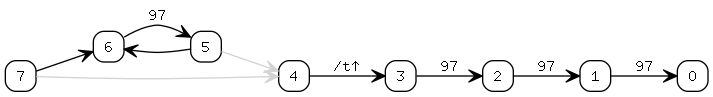
\includegraphics[width=\linewidth]{img/tnfa.pdf}
\caption{
TNFA construction.
}
\end{figure}




\begin{figure*}
\begin{multicols}{2}

    \begin{algorithm}[H] \DontPrintSemicolon \SetKwProg{Fn}{}{}{} \SetAlgoInsideSkip{medskip}
    \Fn {$\underline{match (\XN, \alpha_1 \dots \alpha_n)} \smallskip$} {
        $(\Sigma, T, P, Q, F, q_0, T, \Delta) = \XN$ \;
        $X = closure(\{ (\bot, q_0, \epsilon, t_0) \}, F, \Delta)$ \;
        $(X, B, D) = step(0, X, B, D)$ \;

        \BlankLine
        \For {$i = \overline{1,n}$} {
            $X = reach(X, \Delta, \alpha_i)$ \;
            $X = closure(X, B, D)$ \;
            $(X, B, D) = step(i, X, B, D)$ \;
        }

        \BlankLine
        \lIf {$\exists (\Xund, p, \Xund, t) \in X \mid p \in F$} {
            \Return $t$
        } \lElse {
            \Return $\bot$
        }
    }
    \end{algorithm}


    \begin{algorithm}[H] \DontPrintSemicolon \SetKwProg{Fn}{}{}{} \SetAlgoInsideSkip{medskip}
    \Fn {$\underline{reach (X, \alpha)} \smallskip$} {
        \Return $\{ (p, p', \epsilon, t) \mid$ \;
        $\qquad (\Xund, p, \Xund, t) \in X \wedge
            (p, \alpha, \epsilon, p') \in \Delta^\Sigma \}$
    }
    \end{algorithm}


\iffalse
    \begin{algorithm}[H] \DontPrintSemicolon \SetKwProg{Fn}{}{}{} \SetAlgoInsideSkip{medskip}
    \Fn {$\underline{closure(k, X, B, D)} \smallskip$} {

        $Y = \emptyset$ \;
        \For {$x \in X$} {
            Y = $rclosure (x, Y, B, D)$
        }

        \Return $Y$ \;
    }
    \end{algorithm}


    \begin{algorithm}[H] \DontPrintSemicolon \SetKwProg{Fn}{}{}{} \SetAlgoInsideSkip{medskip}
    \Fn {$\underline{rclosure(x, Y, B, D)} \smallskip$} {
        $(q, p, u, t) = x$ \;
        \If {unmarked $p$} {
        mark $p$ \;

        \If {$p \in F \vee \exists (p, \alpha, \Xund, \Xund) \in \Delta^\Sigma$} {
            \If {$\nexists y = (\Xund, p, \Xund, \Xund) \in Y$} {
                $Y = Y \cup \{ x \}$
            } \ElseIf { $less (x, y, B, D)$} {
                $Y = Y \cup \{ x \} \setminus \{ y \}$
            }
        }

        \BlankLine
        \ForEach {$(p, \epsilon, w, p') \in \Delta^\epsilon$} {
            Y = $rclosure ((q, p', u w, t), Y, B, D)$ \;
        }

        unmark $p$ \;
        }
        \Return $Y$ \;
    }
    \end{algorithm}

    \begin{algorithm}[H] \DontPrintSemicolon \SetKwProg{Fn}{}{}{}
    \Fn {$\underline {less (x, y, B, D)} \smallskip$} {
        $(\Xund, \Xund, l) = precedence (x, y, B, D)$ \;
        \Return $l$ \;
    }
    \end{algorithm}
\fi


    \begin{algorithm}[H] \DontPrintSemicolon \SetKwProg{Fn}{}{}{} \SetAlgoInsideSkip{medskip}
    \Fn {$\underline{step(k, X, B, D)} \smallskip$} {
        let $\{ x_i \}_{i=1}^{n} = \{(q_i, p_i, u_i, t_i) \}_{i=1}^{n} = X$

        \BlankLine
        \tcc {update tag values in $X$}
        \For {$i = \overline {1, n}$} {
            $b_1 \dots b_m = u_i$ \;
            \lFor {$j = \overline{1, m}$} {
                $t_i[b_j] = k$
            }
        }

        \BlankLine
        \tcc {update $B$ and $D$ matrices}
        \For {$i = \overline {1, n}$} {
            \For {$j = \overline {1, n}$} {
                $(h_1, h_2, l) = precedence (x_i, x_j, B, D)$ \;
                $B' [p_i] [p_j] = h_1, \; D' [p_i] [p_j] = l$ \;
                $B' [p_j] [p_i] = h_2, \; D' [p_j] [p_i] = -l$ \;
            }
        }

        \BlankLine
        \Return $(X, B', D')$ \;
    }
    \end{algorithm}

    \columnbreak


    \begin{algorithm}[H] \DontPrintSemicolon \SetKwProg{Fn}{}{}{}
    \Fn {$\underline {precedence (x_1, x_2, B, D)} \smallskip$} {
        $(q_1, \Xund, a_1 \dots a_n, \Xund) = x_1$ \;
        $(q_2, \Xund, b_1 \dots b_m, \Xund) = x_2$ \;
        $k = 1, \; h_1 = h_2 = \infty, \; l = 0$ \;

        \BlankLine
        \tcc {if fork frame, find fork}
        \If { $q_1 = q_2$ } {
            \While {$k < min (n, m)$ and $a_k = b_k$} {
              $k = k + 1$
            }
        }

        \BlankLine
        \tcc {longest-precedence}
        \If { $q_1 = q_2$ } {
            $h_1 = h_2 = height (a_{k-1})$
        } \ElseIf {$k > 1$} {
            $h_1 = B [q_1] [q_2], \; h_2 = B [q_2] [q_1]$
        }
        \lFor {$i = \overline{k, n}$} {
            $h_1 = min (h_1, height (a_i))$
        }
        \lFor {$i = \overline{k, m}$} {
            $h_2 = min (h_2, height (b_i))$
        }
        \lIf {$h_1 > h_2$} {\Return $(h_1, h_2, -1)$}
        \lIf {$h_1 < h_2$} {\Return $(h_1, h_2, 1)$}

        \BlankLine
        \tcc {leftmost-precedence}
        \If { $q_1 = q_2$ } {
            \lIf {$k = n = m$} { $l = 0$ }
            \lElseIf {$k = n$} { $l = -1$ }
            \lElseIf {$k = m$} { $l = 1$ }
            \lElseIf {$a_k mod 2 \equiv 0$} { $l = -1$ }
            \lElseIf {$b_k mod 2 \equiv 0$} { $l = 1$ }
            \lElseIf {$a_k > b_k$} { $l = -1$ }
            \lElseIf {$a_k < b_k$} { $l = 1$ }
        } \Else {
            $l = D [q_1] [q_2]$
        }
        \Return $(h_1, h_2, l)$
    }
    \end{algorithm}

\end{multicols}
\begin{center}
\caption{Matching algorithm.}
\end{center}
\end{figure*}


\begin{figure*}
\begin{multicols}{2}

    \begin{algorithm}[H] \DontPrintSemicolon \SetKwProg{Fn}{}{}{} \SetAlgoInsideSkip{medskip}
    \Fn {$\underline{closure \Xund goldberg \Xund radzik(X, F, \Delta)} \smallskip$} {
        empty stacks $topsort$, $newpass$ \;
        $result(q) \equiv \bot$ \;
        $status(q) \equiv \mathit{OFFSTACK}$ \;
        \For {$(q, x) \in X$} {
            $relax(q, x, result, topsort)$ \;
        }
        \While {$topsort$ is not empty} {
            \While {$topsort$ is not empty} {
                $q = pop(topsort)$ \;

                \If {$status(q) = \mathit{TOPSORT}$} {
                    $push(newpass, n)$ \;
                } \ElseIf {$status(q) = \mathit{NEWPASS}$} {
                    $status(q) = \mathit{TOPSORT}$ \;
                    $push(topsort, q)$ \;
                    $scan(q, result, topsort)$ \;
                }
            }
            \While {$newpass$ is not empty} {
                $q = pop(newpass)$ \;
                $scan(q, result, topsort)$ \;
                $status(q) = \mathit{OFFSTACK}$ \;
            }
        }
        \Return $\big\{ (q, x) \mid x = result(q) \; \wedge$ \;
        $\hspace{6em} \big(q \in F \vee \exists (p, \alpha, \Xund, \Xund) \in \Delta^\Sigma \big) \big\}$ \;
    }
    \end{algorithm}

    \columnbreak

    \begin{algorithm}[H] \DontPrintSemicolon \SetKwProg{Fn}{}{}{} \SetAlgoInsideSkip{medskip}
    \Fn {$\underline{scan(q, result, topsort)} \smallskip$} {
        \ForEach {outgoing arc $(q, \epsilon, \chi, p) \in \Delta$} {
            $x = result(q) \chi$ \;
            $relax(p, x, result, topsort)$ \;
        }
    }
    \end{algorithm}


    \begin{algorithm}[H] \DontPrintSemicolon \SetKwProg{Fn}{}{}{} \SetAlgoInsideSkip{medskip}
    \Fn {$\underline{relax(q, x, result, topsort, B, D)} \smallskip$} {
        $(\Xund, \Xund, l) = precedence (x, result(q), B, D)$ \;
        \If {$l = -1$} {
            $result(q) = x$ \;
            \If {$status(q) \neq \mathit{TOPSORT}$} {
                $push(topsort, q)$ \;
                $status(q) = \mathit{NEWPASS}$ \;
            }
        }
    }
    \end{algorithm}

\end{multicols}
\begin{center}
\caption{GOR1.}
\end{center}
\end{figure*}


\clearpage
\pagebreak

\section{GOR1 correcness proof}

For a given RT $r$,
we say that PE $\alpha$ is \emph{minimal} if $\alpha = PE(t)$ for some minimal $t \in PT(r)$,
and we say that path $\pi$ in TNFA $F(r)$ is \emph{minimal} if $\pi$ induces a minimal PE.

GOR1 correctness proof consists of two parts.
First, we get rid of $\epsilon$-loops by showing that,
on one hand, minmal paths do not contain $\epsilon$-loops,
and on the other hand, GOR1 cancels all paths which contain $\epsilon$-loops.
Second, for paths without $\epsilon$-loops we show right distributivity of path comparison over path concatenation.
The proofs make use of the TNFA nested structure
and the fact that each sub-TNFA is has a unique entry and exit states.
TNFA construct for all possible types of RT are shown on the fugure below.



\begin{figure}\label{fig_gor1}
\includegraphics[width=\linewidth]{img/gor1.pdf}
\caption{
Sub-TNFA for individual sub-RT with submatch groups: \\
(a) -- union, (b) -- product, (c), (d) -- bounded repetition, (e), (f) -- unbounded repetition.
}
\end{figure}

    \begin{XLem}\label{gor1_path_containment}
    Let $r$ be a RE, $\pi = q_1 \overset {\alpha} {\rightsquigarrow} q_2$ a tagged path in TNFA $F(r)$,
    where $\alpha \neq \epsilon$,
    and $h = minht (\alpha)$ the minimal tag height on path $\pi$.
    The following statements are true:
    \begin{enumerate}
        \item There is a position $p$ of length $|p| = h$
            such that $\pi$ fully lies inside of subautomaton $F(r|_p)$.

        \item There no position $p$ of length $|p| > h$
            such that $\pi$ fully lies inside of subautomaton $F(r|_p)$.
    \end{enumerate}
    Proof.
    Obvious from TNFA construction.
    $\square$
    \end{XLem}




    \begin{XLem}\label{gor1_minpaths}
    Minimal paths do not contain tagged $\epsilon$-loops.
    \\
    Proof.

    Suppose, on the contrary, that $\pi$ is a minimal path in TNFA $F(r)$, and that $\pi$ contains at least one $\epsilon$-loop.
    Consider the \emph{last} $\epsilon$-loop in $\pi$:
    it can only come from sub-TNFA of the form $F\big( (i, \Xund, (i_1, \Xund, r_1)^{n,\infty}) \big)$ where $n \geq 0$,
    as this is the only looping TNFA construct.
    Let $w_n$ be the final state of sub-TNFA $F\big( (i_1, \Xund, r_1) \big)$
    as shown on figure \ref{fig_gor1} (e) -- (f).
    Then $\pi$ can be represented as
    $\pi = \pi_1 \pi_2 \pi_3$, where $\pi_2$ is the $\epsilon$-loop:
    $\pi_1 = q_0 \overset {u | \alpha} {\rightsquigarrow} w_n$ and
    $\pi_2 = w_n \overset {\epsilon | \beta} {\rightsquigarrow} w_n$ and
    $\pi_3 = w_n \overset {v | \gamma} {\rightsquigarrow} q_f$.
    Consider path $\pi' = \pi_1 \pi_3$ that is obtained from $\pi$ by removing $\pi_2$.
    It consumes the same input string $uv$ as $\pi$,
    therefore PE transduced by $\pi$ and $\pi'$ are comparable: $\alpha \beta \gamma, \alpha \gamma \in PE(r, uv)$.
    Let $j$ be the total number of repetitions through $F\big( (i_1, \Xund, r_1) \big)$,
    and let $i$ be the index of the $\epsilon$-loop repetition.

    First case: $i = j$.
    In this case fork of $\alpha \beta \gamma$ and $\alpha \gamma$ happens immediately after $(i-1)$-th repetition:
    %
    \begin{alignat*}{10}
        \alpha \beta \gamma &= x_0 \Xl_{h-1} \;&&\; \Xl_h x_1 \Xr_h \hdots \Xl_h x_{i-1} \Xr_h \;&&\big|\; \Xl_h x_{i} \Xr_h \;&&\; \Xr_{h-1} x_{j+1} \\[-0.5em]
        \alpha \gamma       &= x_0 \Xl_{h-1} \;&&\; \Xl_h x_1 \Xr_h \hdots \Xl_h x_{i-1} \Xr_h \;&&\big|\;                   \;&&\; \Xr_{h-1} x_{j+1}
    \end{alignat*}
    %
    It must be $\alpha \beta \gamma \sim \alpha \gamma$,
    because $minht (\beta) = h > h - 1 = minht (first (\gamma))$,
    so at the fork frame $k$ we have $\rho_k = \rho'_k \leq h - 1$.
    %
    Furthermore, it must be $\alpha \gamma \subset \alpha \beta \gamma$,
    because $first (\gamma) = \Xr < \Xl = first (\beta)$.

    Second case: $i < j$.
    In this case $(i + 1)$-th repetition cannot be an $\epsilon$-loop
    (because we assumed that $i$-th repetition is the \emph{last} $\epsilon$-loop),
    therefore
    fork of $\alpha \beta \gamma$ and $\alpha \gamma$ happens
    inside of $i$-th repetition of $\alpha \beta \gamma$
    and $(i + 1)$-th repetition of $\alpha \gamma$:
    %
    \begin{alignat*}{10}
        \alpha \beta \gamma &= x_0 \Xl_{h-1} \;&&\; \Xl_h x_1 \Xr_h \hdots \Xl_h x_{i-1} \Xr_h \Xl_h y_1 \;&&\big|\; y_2 \Xr_h \Xl_h x_{i+1} \Xr_h && \Xl_h x_{i+2} \Xr_h \hdots \Xl_h x_j \Xr_h \;&&\; \Xr_{h-1} x_{j+1} \\[-0.5em]
        \alpha \gamma       &= x_0 \Xl_{h-1} \;&&\; \Xl_h x_1 \Xr_h \hdots \Xl_h x_{i-1} \Xr_h \Xl_h y_1 \;&&\big|\; y_3 \Xr_h                     && \Xl_h x_{i+2} \Xr_h \hdots \Xl_h x_j \Xr_h \;&&\; \Xr_{h-1} x_{j+1}
    \end{alignat*}
    %
    In this case
    fork frame of $\alpha \beta \gamma$ contains $y_2 \Xr_h \Xl_h$ fragment, because $y_2$ is part of the $\epsilon$-loop.
    But the fork frame of $\alpha \gamma$ ends inside of $y_3$, because $(i+1)$-th repetiton is not an $\epsilon$-loop and must contain alphabet symbols.
    Therefore at the fork frame $k$ we have $\rho_k = h$ and $\rho'_k > h$.
    All subsequent frames $l > k$ are identical,
    so either $\rho_l = \rho'_l = h'$ (if $l$-th frame contains parentheses of height $h' \leq h$),
    or else $\rho_l = \rho_k$ and $\rho'_l = \rho'_k$.
    Consequently $\alpha \gamma \sqsubset \alpha \beta \gamma$.

    In both cases $\alpha \gamma < \alpha \beta \gamma$,
    which contradicts the fact that $\pi$ is a minimal path.
    $\square$
    \end{XLem}



    \begin{XLem}\label{gor1_loops}
    GOR1 discards paths with tagged $\epsilon$-loops.
    \\
    Proof.

    GOR1 finds non-looping paths before their looping counterparts,
    as it uses depth-first search to explore new paths and prunes ambiguous paths
    immediately after exploring transitions to the join state.
    So for each TNFA state, the first path to be found is a path without $\epsilon$-loops.
    We will show that once GOR1 has found a path without $\epsilon$-loops,
    it will never prefer a path with an $\epsilon$-loop
    (though of course it might prefer some other path without $\epsilon$-loops).

    The only TNFA construct that has a loop is unbounded repetition
    $F\big( (i, \Xund, (i_1, \Xund, r_1)^{n,\infty}) \big)$ where $n \geq 0$,
    shown on figure \ref{fig_gor1} (e) -- (f).
    Consider arbitrary path $\pi$ that contains
    $\epsilon$-loop through sub-TNFA $F\big( (i_1, \Xund, r_1) \big)$.
    %
    Let $q_1$ be the first state on $\pi$ that belongs to the $\epsilon$-loop.
    %
    Path $\pi$ can be represented as $\pi = \pi_1 \pi_2 \pi_3$, where
    $\pi_1 = q_0 \overset {u | \alpha} {\rightsquigarrow} q_1$ and
    $\pi_2 = q_1 \overset {\epsilon | \beta} {\rightsquigarrow} q_1$ and
    $\pi_3 = q_1 \overset {v | \gamma} {\rightsquigarrow} q_f$.
    %
    By the time GOR1 finds path $\pi_1 \pi_2$,
    it must have already found some other path $\pi'_1 = q_0 \overset {u | \alpha'} {\rightsquigarrow} q_1$ without $\epsilon$-loops.
    There are two possible cases: either $\alpha' = \alpha$, or $\alpha' < \alpha$.
    We will show that in both cases $\alpha' < \alpha \gamma$
    and consequently, GOR1 prefers the path without the $\epsilon$-loop.
    Let $k$ be the index of the last frame
    and $\big( (\rho_1, \hdots, \rho_k), (\rho'_1, \hdots, \rho'_k) \big) = traces (\alpha', \alpha \gamma)$.

    First case: $\alpha' = \alpha$.
    Because $\alpha$ is a proper prefix of $\alpha \gamma$,
    fork happens at the last frame and we have
    $\rho_k = lastht(\alpha)$ and
    $\rho'_k = min (lastht(\alpha), minht(\gamma))$.
    If $lastht(\alpha) > minht(\gamma)$, then $\rho_k > \rho'_k$ and $\alpha \sqsubset \alpha \gamma$.
    Otherwise $\rho_k = \rho'_k$ and $\alpha \sim \alpha \gamma$,
    and we have $first(\alpha \backslash \alpha \gamma) = \bot$ and $first(\alpha \gamma \backslash \alpha) \neq \bot$,
    therefore $\alpha \subset \alpha \gamma$.
    In both cases $\alpha < \alpha \gamma$.

    Second case: $\alpha' < \alpha$.
    Let $\big( (\sigma_1, \hdots, \sigma_k), (\sigma'_1, \hdots, \sigma'_k) \big) = traces (\alpha', \alpha)$.
    We have $\rho_k = \sigma_k$ and $\rho'_k = min (\sigma'_k, minht(\gamma)) \leq \sigma_k$.
    If $minht(\gamma) < \sigma'_k$ then $\rho_k > \rho'_k$ and $\alpha' \sqsubset \alpha \gamma$.
    Otherwise $\rho'_k = \sigma'_k$.
    If $\alpha' \sqsubset \alpha$ then $\alpha' \sqsubset \alpha \gamma$.
    Otherwise $\alpha' \sim \alpha$ and $\alpha' \subset \alpha$.
    None of $\alpha$ and $\alpha'$ is a proper prefix of the other,
    because otherwise the longer path has an $\epsilon$-loop through $q_1$, which contradicts our assumption about $\pi_1$ and $\pi'_1$.
    Therefore $first (\alpha' \backslash \alpha) = first (\alpha' \backslash \alpha \gamma)$
    and $first (\alpha \backslash \alpha') = first (\alpha \gamma \backslash \alpha')$.
    Consequently $\alpha' \subset \alpha \implies \alpha' \subset \alpha \gamma$.
    Thus $\alpha' < \alpha \gamma$.
    $\square$
    \end{XLem}





    \begin{XLem} \emph{(Right distributivity of path comparison over path concatenation for $\epsilon$-loop free paths.)}
    Let
    $\pi_\alpha = q_0 \overset {u | \alpha} {\rightsquigarrow} q_1$ and
    $\pi_\beta  = q_0 \overset {u | \beta}  {\rightsquigarrow} q_1$
    be ambiguous paths in TNFA $F(r)$
    and $\pi_\gamma = q_1 \overset {\epsilon | \gamma} {\rightsquigarrow} q_2$
    their common $\epsilon$-suffix,
    such that paths $\pi_\alpha$, $\pi_\beta$
    and the extended paths $\pi_\alpha \pi_\gamma$, $\pi_\beta \pi_\gamma$
    are all free from $\epsilon$-loops.
    Then $\alpha < \beta \implies \alpha \gamma < \beta \gamma$.
    \\
    Proof.

    Let $k = |u|$ be the number of frames in $\alpha$ and $\beta$.
    Let
    $\big( (\rho_1, \hdots, \rho_k),$ $(\rho'_1, \hdots, \rho'_k) \big) = traces (\alpha, \beta)$ and
    $\big( (\sigma_1, \hdots, \sigma_k),$ $(\sigma'_1, \hdots, \sigma'_k) \big) = traces (\alpha \gamma, \beta \gamma)$.
    Obviously for frames $i < k$ we have $\rho_i = \sigma_i$ and $\rho'_i = \sigma'_i$,
    and for the last frame $k$ we have
    $\sigma_k = min (\rho_k, minht (\gamma))$ and
    $\sigma'_k = min (\rho'_k, minht (\gamma))$.
    Consider two possible cases.

    First case: $\alpha \sim \beta \wedge \alpha \subset \beta$.
    %
    We show that $\alpha \gamma \sim \beta \gamma \wedge \alpha \gamma \subset \beta \gamma$.
    %
    We have $\rho_i = \rho'_i \; \forall i$, therefore
    $\sigma_i = \sigma'_i \; \forall i$ and consequently $\alpha \gamma \sim \beta \gamma$.
    Let
    $x = first (\alpha \backslash \beta)$,
    $y = first (\beta \backslash \alpha)$,
    $x' = first (\alpha \backslash \beta \gamma)$ and
    $y' = first (\beta \backslash \alpha \gamma)$.
    None of $\pi_\alpha$ and $\pi_\beta$ is a proper prefix of another,
    otherwise the longer path must contain $\epsilon$-loop through $q_1$
    (because $\alpha$ and $\beta$ have the same number of frames).
    Consequently $x = x'$ and $y = y'$, and we have
    $\alpha \subset \beta$
    $\implies$
    $x < y$
    $\implies$
    $x' < y'$
    $\implies$
    $\alpha \gamma \subset \beta \gamma$.

    Second case: $\alpha \sqsubset \beta$.
    We show that $\alpha \gamma \sqsubset \beta \gamma$.
    %
    If $\rho_k = \rho'_k$ then $\sigma_k = \sigma'_k$
    and obviously $\alpha \gamma \sqsubset \beta \gamma$.
    Else it must be $\rho_k > \rho'_k$.
    In this case, if $minht (\gamma) > \rho'_k$, then $\sigma_k > \sigma'_k$ and again $\alpha \gamma \sqsubset \beta \gamma$.
    Else $minht (\gamma) \leq \rho'_k$ and $\sigma_k = \sigma'_k$.
    In this case, if $k > 1$ and $\rho_{k-1} > \rho'_{k-1}$ then again $\alpha \gamma \sqsubset \beta \gamma$.
    %
    In other words, the only possible case when $\gamma$ can change comparison result is
    when at the last frame we have $\rho_k > \rho'_k$,
    the appended suffix $\gamma$ contains parentheses with low height $minht (\gamma) \leq \rho'_k$
    (so that $\sigma_k = \sigma'_k$),
    and the previous frame doesn't exist
    or compares differently from the last frame: $k = 1$ or $\rho_{k-1} \leq \rho'_{k-1}$.
    We show that in this case the extended path $\pi_\beta \pi_\gamma$ must contain $\epsilon$-loop,
    which contradicts to the lemma condiitons.

    Consider the fragments of paths $\pi_\alpha$ and $\pi_\beta$ from fork to join,
    including (if it exists) the $\epsilon$-transition to the fork state:
    $\pi_\alpha' = q_2 \overset {u | \alpha'} {\rightsquigarrow} q_1$ and
    $\pi_\beta' = q_2 \overset {u | \beta'} {\rightsquigarrow} q_1$.
    We know that $minht (\alpha') = \rho_k$.
%    (because $\rho_k$ is set to the minimal parenthesis height on the path from fork to join).
    Therefore by lemma \ref{gor1_path_containment}
    we know that $\pi_\alpha'$ is contained in a subautomaton $f$ of height $\rho_k$.
    Likewise we know that $\pi_\beta'$ is not contained in $f$, because $minht (\beta') = \rho'_k < \rho_k$.
    %
    Let $\pi_\beta''$ be the part of $\pi_\beta'$ containing the last $k$-th frame,
    and note the following:
    \begin{enumerate}
        \item[(a)] the start state of $\pi_\beta''$ must be contained in $f$
            (because by our assumption
            either $k = 1$ and then start state of $\pi_\beta''$ is the fork state,
            or $\rho_{k-1} \leq \rho'_{k-1}$ which implies $\rho'_{k-1} \geq \rho_k$
            and then all but the last frames of $\pi_\beta'$ must be contained in $f$)
        \item[(b)] $\pi$ cannot be contained in $f$
            (because by our assumption $\rho_k > \rho'_k$)
        \item[(c)] the end state of $\pi_\beta''$ is contained in $f$
            (because it's the join state $q_1$ of $\pi_\alpha'$ and $\pi_\beta'$)
        \item[(d)] $\pi_\gamma$ is not contained in $f$
            (because by our assumption $minht (\gamma) \leq \rho'_k$ and consequently $minht (\gamma) < \rho_k$)
    \end{enumerate}
    %
    Put together, items (a) - (d) mean that the $\epsilon$-path $\pi_\beta'' \pi_\gamma$
    first leaves subautomaton $f$, then re-enters $f$, and then leaves $f$ second time.
    Because $f$ has a unique exit state, this means that $\pi_\beta'' \pi_\gamma$ contains $\epsilon$-loop
    through the exit state of $f$, which contradicts lemma conditions.
    (Effectively it means that $\pi_\beta \pi_\gamma$ is non-minimal and would be discarded by GOR1 anyway.)
%   Note that $\pi_\beta'$ itself does not necessarily contain $\epsilon$-loop.
    %
    $\square$
    \end{XLem}




\section{Matching algorithm}

The final algorithm, complexity estimates.

\section{Conclusions}

\end{document}

